\documentclass[a4paper,12pt]{scrartcl}
\usepackage[ngerman]{babel}
\usepackage[utf8]{inputenc}
\usepackage{pdfpages}
\usepackage{scrpage2}
\usepackage{graphicx}
\usepackage{booktabs}
%\usepackage{times}
%\usepackage{helvet}
\usepackage[T1]{fontenc}
\usepackage{fourier}
\pdfcompresslevel=9
\usepackage[%
    %%% general options
    pdftex=true,      %% sets up hyperref for use with the pdftex program
    %plainpages=false, %% set it to false, if pdflatex complains: ``destination with same identifier already exists''
    %
    %%% extension options
    colorlinks=true,   %% turn on colored links (true is better for on-screen reading, false is better for printout versions)
    %
    %%% PDF-specific display options
    bookmarks=false,          %% if true, generate PDF bookmarks (requires two passes of pdflatex)
    bookmarksopen=false,     %% if true, show all PDF bookmarks expanded
    bookmarksnumbered=false, %% if true, add the section numbers to the bookmarks
    %pdfstartpage={1},        %% determines, on which page the PDF file is opened
    pdfpagemode=None         %% None, UseOutlines (=show bookmarks), UseThumbs (show thumbnails), FullScreen
]{hyperref}
\hypersetup{
    pdftitle={Lebenslauf}, %%
    pdfauthor={Michael Durrer}, %%
    pdfsubject={Bewerbung}, %%
    pdfcreator={Michael Durrer}, %% 
    pdfproducer={pdflatex}, %%
    pdfkeywords={Bewebung Lebenslauf Michael Durrer} %%
}

% Zeilenabstände
\newlength{\defbaselineskip}
\setlength{\defbaselineskip}{\baselineskip}
\newcommand{\setlinespacing[1]}%
%\newcommand{\ts}{\textsuperscript} % ts Scripting Idee
%\setlength{\baselineskip}{#1 \defbaselineskip}
\newcommand{\singlespacing}{\setlength{\baselineskip}{\defbaselineskip}}
\newcommand{\Zeilenabstand}{\setlength{\baselineskip}{1.5\defbaselineskip}}
\newcommand{\litabstand}{\setlength{\baselineskip}{1.0\defbaselineskip}}
\newcommand{\erkabstand}{\setlength{\baselineskip}{0.2\defbaselineskip}}
\newcommand{\tst}{\setlength{\baselineskip}{2.0\defbaselineskip}}
% Ende Zeilenabstände

\newcommand{\tocka}{\textbullet}
\newcommand{\nz}{~\\[\medskipamount]}
\newcommand{\nzb}{~\\[\bigskipamount]}
\newcommand{\dateitem}[2]{\hspace*{0.5cm}\parbox[t]{4cm}{#1}\hspace*{0.5cm}\parbox[t]{10cm}{#2}~\\[\medskipamount]}
\newcommand{\textitem}[2]{\parbox[t]{4.5cm}{#1}\hspace*{0.5cm}\parbox[t]{10cm}{#2}~\\[\medskipamount]}
\newcommand{\headitem}[1]{\nzb\nzb{\sc #1}\\\erkabstand \rule{\textwidth}{0.5pt}\nzb}

\begin{document}
\parskip 0.0em
\parindent=0pt
\setlength{\unitlength}{1mm}
\pagestyle{scrheadings}
\cfoot{
    \centering Michael Durrer~\tocka~Aarburgerstrasse 197~\tocka~4600 Olten~\tocka~Tel: +41 (0)76 450 0770~\tocka~Email: michael.durrer@gmail.com
}

\begin{center}
{\Huge \sc lebenslauf}
\end{center}

%%%%%%%% NEXT SECTION %%%%%%%%%%%%%%%%
%{\sc Pers\"{o}nliche Anagaben}\\\erkabstand \rule{\textwidth}{0.5pt}\nzb
\headitem{pers\"onliche angaben}
%\hspace*{1.5cm}
\parbox{30em}{
\begin{minipage}{9.4cm}
Name: Michael Durrer\nz
Familienstand: ledig\nz
Staatsangeh\"{o}rigkeit: Schweiz\nz
Geburtsdatum: 27.3.1987\nz
Geburtsort: Zofingen
\end{minipage} \hfill
\begin{minipage}{0.0cm}
\begin{flushright}
%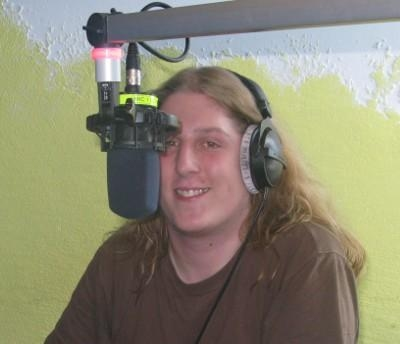
\includegraphics[height=4cm]{portrait.png}
\end{flushright}
\end{minipage}
}\nzb

%%%%%%%% NEXT SECTION %%%%%%%%%%%%%%%%
\headitem{schulische ausbildung}
\dateitem{2003 -- 2004}{Berufswahlschule / 10. Schuljahr, Aarburg}
\dateitem{1999 -- 2003}{Bezirksschule, Rothrist}
\dateit\dateitem{1994 -- 1999}{Primarschule, Rothrist}

%Abschluss: Oberstufe}
%%%%%%%% NEXT SECTION %%%%%%%%%%%%%%%%
\headitem{berufliche ausbildung}
\dateitem{2004 -- 2008}{Lehre zum Fachinformatiker (Anwendungsentwickler und Systemtechniker), \textbf{BerufsBildungBaden} in \textbf{Baden}}
%%%%%%%% NEXT SECTION %%%%%%%%%%%%%%%%
\headitem{berufspraxis}
\dateitem{01/2010 --heute}{Verschiedene Flyer-Arbeiten für E-Zigaretten-Händler, Aufbau meines Freelance-Unternehmens Aikyatchi}
\dateitem{01/2010 -- 10/2010}{Informatiker (Serververwaltung, Webseiten-Entwicklung) und Studiotechniker/Redaktor (Abmischen, Erstellung und Bearbeitung von Beiträgen, Liveübertragungen) bei \textbf{Kanal K},\textbf{ Aarau}}
\dateitem{12/2008 -- 04/2009}{Weltweiter Kundensupport (deutsch-, englisch- und französischsprachig) für BMC BladeLogic [Serverwaltungssoftware] bei \textbf{ECfOS GmbH}, \textbf{Dietikon}}
\dateitem{09/2008 -- 10/2008}{1\ts{st}-Level-Support bei \textbf{Green.ch}, \textbf{Brugg} }
\dateitem{2007 -- 2008}{Abschluss der Lehre als Systemtechniker (.NET-Entwicklung und IBM DB2- u. MySQL-Datenbankenverwaltung, Logo-Designs u.Ä.) bei \textbf{Weinkellereien Aarau GmbH, \textbf{Buchs und Aarau}}}
\dateitem{2006 -- 2007}{Systemtechniker (Netzwerkverwaltung, kleinere graphische Arbeiten, MacOS X-Umgebungen) bei \textbf{Solutionpark GmbH}, \textbf{Zürich}}
\dateitem{2004 -- 2006}{Applikationsentwickler bei \textbf{Art & Tech AG}, \textbf{Aarau}}
%%%%%%%% NEXT SECTION %%%%%%%%%%%%%%%%
\newpage
\headitem{besondere kenntnisse, interessen und freizeitaktivitäten}
\textitem{Fremdsprachen}{Englisch - Fliessend in Schrift und Sprache\newline Französisch - Nach Schulbildung und autodidaktische Weiterbildung \newline Niederländisch - Mittel bis gut}
\newline
\textitem{Hobbys}{Literatur und Film, Grafik-/Video-Design und -Bearbeitung, Musik machen (MIDI-Keyboard und Gitarre / Fruity Loops u. Cubase 6.x), Engagement in diversen Open Source Projekten}
\newline
\textitem{Projekte}{\begin{itemize}

\item Das Planen und Schreiben meines Sachbuch-Projekts „Entwicklung von Spielen und
Emulatoren unter GNU/Linux“: http://movie.emulator.googlepages.com 
\textit{(Älterer Entwurf liegt als PDF bei)}
\newline 
\item Entwicklung eines modularen Emulators: http://sourceforge.net/projects/mve
\item Entwicklung einer Point'n Click-Adventure Engine mit Python/PyGame
\item Aufbau von sogenannten 'Hackerspaces' in Olten
\end{itemize}

}
%\nzb\nzb
%%%%%%%% NEXT SECTION %%%%%%%%%%%%%%%%
%Weiterbildung:\\\erkabstand \rule{\textwidth}{0.5pt}\nzb
%\dateitem{11/2002 -- 01/2003}{Berufsvorbereitungslehrgang
%im beruflichen Fortbildungszentrum, Selb}\nz
%\nzb\nzb
%%%%%%%% NEXT SECTION %%%%%%%%%%%%%%%%
%Besondere F\"{a}higkeiten\\\erkabstand \rule{\textwidth}{0.5pt}\nzb
%\dateitem{}{Spa\ss{} am Kontakt und Austausch mit Menschen.}\nz
%\dateitem{}{Interesse am politischen Tagesgeschehen.}\nz
\newpage
%%%%%%%% NEXT SECTION %%%%%%%%%%%%%%%%
\begin{center}
{\Huge \sc fachliche kenntnisse}
\end{center}

\headitem{linux mailserver}
\textitem{Mailserver}{Postfix, Exim, Sendmail}
\textitem{Filter}{Spamassassin}
\textitem{Antivirus}{Amavis}
\textitem{Webinterface}{SquirrelMail}
\textitem{User Backend}{MySQL, SQLite, LDAP}

\headitem{linux netzwerk}
\textitem{Webserver}{Apache2}
\textitem{Firewall}{IPTables Skripte, IPCop, DMZ Umgebungen}
\textitem{VPN}{OpenVPN}
\textitem{Heterogenes Netzwerk}{Samba, auch als Domain Controller mit LDAP Backend}
\textitem{\"{U}berwachung}{Nagios, CRON-Jobs (Surveillance-Scripting)}
\textitem{Analyse}{Tcpdump, Ethereal, Wireshark}
\textitem{Verschl\"{u}sselung}{GnuPG}
\textitem{DNS}{Bind9}

\headitem{linux und unix}
\textitem{Distributionen}{Haupts\"achlich Ubuntu, Debian, RPM-basierte Distributionen (Red Hat, Mandriva), MacOS X Snow Lion, Solaris}\nz

\headitem{entwicklung}
\textitem{IDE}{Eclipse, NetBeans, IDLE, Visual Studio .NET}
\textitem{Versionsverwaltung}{Subversion, Concurrent Version System (CVS), Git}
\textitem{Programmiersprachen}{Sehr gut: Python, PHP, C/C++/C#, 6502/6510- und x86-Assembler\newline

Gut: SED, Regexp, Bash-Shell\newline

Grundlagen: Java, Perl, Ruby (On Rails)}
\textitem{Webseiten}{HTML5 (<canvas>-Erfahrung), CSS2, Javascript, AJAX (JQuery), Django, Mambo CMS, typo3 CMS}

\headitem{datenbanken}
MySQL, SQLite, Oracle, MS Access
\newpage
\begin{center}
{\Huge \sc fachliche kenntnisse}
\end{center}


\headitem{windows}
\textitem{Betriebssysteme}{Administration von Windows 7, XP, 2000, ME, 98, 95, Windows Server Installationen}
\textitem{Directory-Management}{Erstellung und Verwaltung von ActiveDirectory-Realms}
\textitem{Officesupport} {Bedienung, Konfiguration und Supportdienstleistung für Microsoft Office sowie LibreOffice}
\textitem{MS Office}{Word, Excel, Access, PowerPoint, Outlook, Visio}

\headitem{groupware}
eGroupWare,phpProjekt\nz

\headitem{virtualisierung}
VMware ESX(i) Server sowie VMware Workstation, KVM, Qemu

\headitem{telekommunikation}
\textitem{VoIP-Telefonsysteme/PBX}{Asterisk}
\headitem{hardware}
\textitem{PC-Bau} {Erfahren in Fehleranalyse, Reparatur, Einkauf}\nz
\textitem{Netzwerk}{Fehleranalyse anhand von Konsolentools und Aufbau/Wartung von heterogenen Netzwerken}
\textitem{Elektrotechnik}{Reparatur von Elektronikgeräten, Erfahrungen mit Raspberry PI, C64 (6510 CPU), Amiga (68xxx CPU) sowie Planung und Umsetzung von Schaltungen}
\newpage
\begin{center}
{\Huge \sc fachliche kenntnisse}
\end{center}
\headitem{multimedia}
\textitem{Grafik}{GIMP, Blender 2.6+, Photoshop CS6, Inkscape, Synfig Studio, Scribus (DTP)}
\textitem{Video}{Final Cut Pro X, Cinerella, Blender 2.6+, VirtualDub, Jahshaka}}
\textitem{Audio und Musik}{Adobe Audition, Fruity Loops, Steinberg Cubase, Linux MultiMedia Studio (LMMS), MIDI-Erfahrung}
\nzb\nzb
Sollten Sie mehr Informationen zu einzelnen Projekten w\"unschen, bin ich gerne dazu bereit, Ihnen diese auf Anfrage zur Verf\"ugung zu stellen.

%Kenntnisgrade:\nz + Grundkenntnisse, ++ fortgeschrittene Kenntnisse,
%+++ sehr gute Kenntnisse\nz

%\begin{tabular}{|l|l|l|l|}
%\hline
% after \\: \hline or \cline{col1-col2} \cline{col3-col4} ...
%\textbf{Gebiet} & \textbf{Teilgebiet} & \textbf{Kenntnisgrad} & \textbf{in Jahren} \\
%\hline
%\hline
%Betriebssysteme & GNU/Linux & +++ & 7 \\ \hline
%& Windows (98,2000,XP) & ++ & 10 \\ \hline
%& Mac OS X & ++ & 2 \\ \hline
%\hline
%Programmiersprachen & Perl & ++ & 3 \\ \hline
%& Phyton & + & 1 \\ \hline
%\hline
%Produkte & MS Office & ++ & 5 \\ \hline
%& OpenOffice & ++ & 3 \\ \hline
%& \LaTeX & ++ & 4 \\ \hline
%\hline
%Sprachen & Deutsch & Muttersprache & -\\ \hline
%& Englisch & verhandlungssicher & - \\ \hline
%& Spanisch & Grundkenntnisse & - \\ \hline
%\end{tabular}
%\nzb

\nzb \nzb

Michael Durrer, Olten, \today
\newpage
\cfoot{}
\setlength{\textwidth}{\paperwidth}
\setlength{\textheight}{\paperheight}
\setlength{\headheight}{0pt}
\setlength{\topmargin}{-94.0pt}
\setlength{\evensidemargin}{-70pt}
\setlength{\oddsidemargin}{-70pt}
\end{document}

